\documentclass[letterpaper,11pt]{article}
\usepackage[spanish, activeacute]{babel}
\usepackage{amsmath,amsfonts,amssymb}
\usepackage{fancyhdr}
\usepackage{fancyvrb}
\usepackage{graphicx}
\usepackage{amsfonts}
\usepackage{enumerate}
\usepackage{multirow}
\usepackage{multicol}
\usepackage{longtable}
\usepackage{hyperref}
\hypersetup{
    colorlinks=true,       % false: boxed links; true: colored links
    linkcolor=red,          % color of internal links (change box color with linkbordercolor)
}
\usepackage[numbered,framed]{matlab-prettifier}
\lstMakeShortInline"
\lstset{
  style              = Matlab-editor,
  escapechar         = ",
  mlshowsectionrules = true,
}

\setlength{\oddsidemargin}{-0.5cm}
\setlength{\evensidemargin}{0cm}
\setlength{\textwidth}{17.5cm}
\setlength{\textheight}{24cm}
\setlength{\topmargin}{-1.7cm}

\title{lab04 521230 2018-1}

\font\bff=cmbx10 at 10truept
\font\lg=cmdunh10 at 10truept
\font\bl=cmss10 at 10truept

\newcommand{\matlab}{{\sc Matlab} }

\newcommand{\header}{\noindent%
{\lg UNIVERSIDAD DE CONCEPCI\'ON}\hfill
\vskip-4truept
\noindent{\bff FACULTAD DE CIENCIAS}\hfill
\vskip-4truept
\noindent{\bff F\'ISICAS Y MATEM\'ATICAS}\hfill
\vskip-4truept
\noindent{\bl DEPARTAMENTO DE INGENIER\'IA MATEM\'ATICA}\hfill
\vskip4truept\hrule\hrule\vskip4truept
\par
}

\begin{document}
\header
\vspace{0.7cm}
\begin{center}
\textbf{\small C\'alculo Num\'erico (521230) - Laboratorio 4}\\
\vspace{0.1cm}
\textbf{\Large INTERPOLACI\'ON EN MATLAB}
\vspace{0.7cm}
\end{center}


Matlab incluye funciones para calcular y manipular funciones interpolantes; entre ellas:

\begin{longtable}{||c|p{0.7\textwidth}||}
\hline
\texttt{vander(x)} 			& Retorna la matriz de Vandermonde de una colecci\'on de abscisas en el vector \texttt{x}.\\
\hline
\texttt{interp1(x,y,xq)}	& Retorna los valores interpolados de una funci\'on que pasa por los puntos de coordenadas \texttt{x,y} en ciertos puntos \texttt{xq}.\\
\hline
\texttt{polyfit(x,y,n)}	& Retorna los coeficientes del polinomio de grado menor o igual a \texttt{n} que mejor se ajusta a los datos \texttt{x} e  \texttt{y}. Para evaluar el polinomio se debe usar \texttt{polyval}. \\
\hline
\texttt{spline(x,y,xq)}	& Retorna los valores interpolados de un spline c\'ubico que pasa por los puntos de coordenadas \texttt{x,y} en ciertos puntos \texttt{xq}.\\
\hline 
\end{longtable}


\section{Interpolaci\'on polinomial}
De la teor\'ia sabemos que dado un conjunto de $n+1$ puntos $\{(x_i,y_i)\}_{i=0}^{n}$ que no repitan abscisas (esto es, $i \neq j \implies x_i \neq x_j$), existe un \'unico polinomio interpolante de grado menor o igual a $n$. Para el c\'alculo de este polinomio se debe resolver un sistema de ecuaciones el cual se puede estructurar dependiendo de la base del espacio de polinomios que se elija (base can\'onica de monomios o base de polinomios de Lagrange). 

El rutero \href{ftp://ftp.ing-mat.udec.cl/pub/ing-mat/asignaturas/521230/ejercicios/2018-1/interpolacion1.m}{interpolacion1.m} muestra la aproximaci\'on y gr\'afica de un polinomio interpolante para un conjunto de puntos muestreados de la funci\'on \texttt{sin}. Comente cada instrucci\'on que se presenta en este programa.

\section{Polinomios de Lagrange}

%El párrafo de la discordia
%Utilizar la matriz de Vandermonde para muchos puntos no es muy buena idea porque esa matriz es muy sensible a perturbaciones en los datos. Una alternativa es utilizar los polinomios de Lagrange: En general, un polinomio interpolante tiene la forma

Utilizar la matriz de Vandermonde para muchos puntos no es muy buena idea porque esta puede llevar a errores de representaci\'on en la memoria del computador (overflow, underflow o redondeo). Una alternativa, para evitar resolver un problema que involucre a una matriz de Vandermonde, es utilizar los polinomios de Lagrange. En general, un polinomio interpolante tiene la forma
$$\displaystyle
p(x)=\sum_{k=0}^{n} \prod_{\substack{i=0\\i\neq k}}^n \frac{x-x_i}{x_k-x_i} \, y_k,
$$
tal interpolaci\'on se puede evaluar con la siguiente
\href{ftp://ftp.ing-mat.udec.cl/pub/ing-mat/asignaturas/521230/ejercicios/2018-1/polyinterp.m}{funci\'on}
\begin{lstlisting}
function v = polyinterp(x,y,u)
    n = length(x);
    v = zeros(size(u));
    for k = 1:n
      w = ones(size(u));
      for i = 1:n
        if i ~= k
          w = (u-x(i))./(x(k)-x(i)).*w;
        end
      end
      v = v + w*y(k);
    end
\end{lstlisting}
donde el conjunto de puntos de interpolaci\'on tienen coordenadas representadas en los vectores \texttt{x,y}, las abscisas de los puntos interpolados son los elementos de \texttt{u} y las ordenadas de los puntos interpolados son los elementos de la salida \texttt{v}. Las siguientes instrucciones nos permiten graficar el polinomio interpolante de una funci\'on.
\begin{lstlisting}
  x=-2:1:2;
  y=sin(x.^3);
  figure;
  plot(x,y,'o'); hold on
  t=-2:0.01:2;
  plot(t,polyinterp(x,y,t),'r');
  plot(t,sin(t.^3),'g');
  legend('Puntos','Interpolacion','Curva original');
\end{lstlisting}

\section{Ejemplos}

Los siguientes ejemplos muestran ejecuciones de las funciones de interpolaci\'on


\begin{multicols}{2}
\begin{enumerate}
\item C\'alculo y gr\'afica de un polinomio interpolante con \texttt{polyinterp}
\begin{verbatim}
x=0:1:10;
y=exp(x.^2);
t=-10:0.01:10;
v=polyinterp(x,y,t);
figure;
plot(x,y,'o',t,exp(t.^2),'-',t,v,'--');
\end{verbatim}

\item C\'alculo de los coeficientes de un polinomio con \texttt{vander}
\begin{verbatim}
x=1:10;
y=sin(x.^2);
coef=vander(x)\y
\end{verbatim}

\item Gr\'afica de un spline con \texttt{spline}.
\begin{verbatim}
x = 0:10;
y = sin(x);
xx = 0:.25:10;
yy = spline(x,y,xx);
plot(x,y,'o',xx,yy,'--')
\end{verbatim}
\end{enumerate}
\end{multicols}


\section{Ajuste de curvas por m\'inimos cuadrados}

Un problema de ajuste lineal de datos es buscar una funci\'on $f:\mathbb{R}\times\mathbb{R}^n \rightarrow \mathbb{R}$ donde 
$$
f(t, \mathbf{x}) = x_1 \, \phi_1(t) + x_2 \, \phi_2(t) + \dots + x_n \, \phi_n(t).
$$
Por ejemplo, un problema de ajuste polinomial consiste en buscar una funci\'on
$$
f(t, \mathbf{x}) =x_1 + x_2 \, t + \dots + x_n \, t^{n-1} 
$$
que se ajuste a los datos $\{(t_i,y_i)\}_{i=1}^n$, esto induce el sistema  $\mathbf{A} \mathbf{x} = \mathbf{b}$, donde $\mathbf{A} = (\phi_j(t_i))_{i,j=1}^n$, y $\mathbf{b} = (y_i)_{i=1}^n$. Probamos que tal sistema de ecuaciones tiene como soluci\'on \textbf{en el sentido de los m\'inimos cuadrados} a
$$
\mathbf{x} = (\mathbf{A}^\mathrm{T} \mathbf{A})^{-1} \mathbf{A}^\mathrm{T} \mathbf{b},.
$$

Matlab posee las siguientes funciones para calcular y evaluar ajustes de polinomios
\begin{longtable}{||c|p{0.7\textwidth}||}
\hline
\texttt{p=polyfit(x,y,n)} 
	& Encuentra los coeficientes de un polinomio \texttt{p} de grado menor o igual a \texttt{n} que se ajusta a los puntos de coordenadas \texttt{x, y} en el sentido de los m\'inimos cuadrados.
\\
\hline
\texttt{y=polyval(p,x)} 
	& Retorna los valores de un polinomio \texttt{p} evualuado en las componentes del vector \texttt{x}.\\
\hline
\end{longtable}

En este curso, de hallarnos con un modelo de ajuste no lineal, lo transformaremos en uno lineal usando funciones incluidas en Matlab.
Por ejemplo, si nos interesa ajustar los puntos 
\begin{lstlisting}
t=[10 20 30 40 50 60 70 80];
y=[1.06 1.33 1.52 1.68 1.81 1.91 2.01 2.11];
\end{lstlisting}
a un modelo no lineal de la forma 
$$
f(t,x)=x_1 \, e^{x_2 \, t},
$$
tomando logaritmo natural a ambos lados lo transformamos en
$$
\ln(f(t,x))= \ln(x_1)+ x_2 \, t,
$$
de donde podemos hallar los par\'ametros de ajuste $x_1$ y $x_2$ mediante
\begin{lstlisting}
p=polyfit(t,log(y),1); % En Matlab el logaritmo natural es log
fprintf('parametro x_2 = %2.3f\n',p(1));
fprintf('parametro x_1 = %3.3f\n',exp(p(2)));
hold on
plot(t,y,'ro')
x=linspace(min(t),max(t),50);
z=exp(p(2))*exp(p(1)*x);
plot(x,z,'b')
xlabel('x')
ylabel('y')
title('Regresion exponencial')
hold off
\end{lstlisting}

Otros modelos que se pueden encontrar al ajustar los puntos \texttt{t} e \texttt{y}
$$
\begin{array}{||c|l||}
  \hline
  \text{Funci\'on}				& \text{Llamada a \texttt{polyfit()}} \\
  \hline
  \displaystyle
  f(t,(x_1,x_2))=x_1\cdot t^{x_2}		& \texttt{p=polyfit(log(t), log(y),1)}\\
  \hline
  \displaystyle
  f(t,(x_1,x_2))=x_1\cdot e^{x_2t}		& \texttt{p=polyfit(t, log(y),1)}\\
  \hline    
  \displaystyle
  f(t,(x_1,x_2))=x_1 \cdot ln(t)+x_2	& \texttt{p=polyfit(log(t),y,1)} \\
  \hline
  \displaystyle
  f(t,(x_1,x_2))=\frac{1}{x_1t+x_2}		& \texttt{p=polyfit(t,1./y,1)}\\ 
  \hline
\end{array}
$$

\subsection{Ejemplos}
                                                                                                                                                                 
Los siguientes ejemplos muestran ejecuciones de las funciones de ajuste de curvas por m\'inimos cuadrados

\begin{enumerate}

\item El siguiente ejemplo muestra el uso de la funci\'on \texttt{polyfit}.
\begin{lstlisting}
  x=[0 1 2 3 4 5 6 7 7.44];
  y=[0 4.03 8.12 14.23 20.33 27.1 34.53 42.63 46.43];
  p=polyfit(x,y,2)
  hold on
  plot(x,y,'ro','markersize',8,'markerfacecolor','r')
  x=linspace(min(x),max(x),50);
  y=polyval(p,x);
  plot(x,y,'b')
  xlabel('x')
  ylabel('y')
  title('Polinomio aproximador')
  hold off
\end{lstlisting}
    
    \item La funci\'on \texttt{mldivide} (alias corto: \texttt{\textbackslash}) utiliza por defecto aproximaciones en el sentido de m\'inimos cuadrados. Este ejemplo es el de un sistema sobredeterminado resuelto en el sentido de los m\'inimos cuadrados
    \begin{lstlisting}
A = [1 2 0; 0 4 3];
b = [8; 18];
x = A\b
    \end{lstlisting}
    
\end{enumerate}

\section{Otros modelos de ajustes lineales no polinomiales}
Similarmente a lo desarrollado en la secci\'on anterior, diversos modelos de funci\'on pueden ajustarse a una serie de puntos.

\subsection{Regresi\'on logit}
Dados dos valores $\beta_0,\beta_1\in\mathbb{R}$, se define la funci\'on log\'istica o logit
$$
\begin{array}{rcl}
\pi:\mathbb{R} & \longrightarrow & \mathbb{R} \\
x & \longmapsto &\displaystyle\frac{e^{\beta_0+\beta_1x}}{1-e^{\beta_0+\beta_1x}} 
\end{array}
$$
mediante algunas operaciones algebraicas puede probarse que
$$
\displaystyle
\pi(x)=\frac{1}{e^{-\beta_0-\beta_1x}-1}, \quad
ln\left(\frac{\pi(x)}{1+\pi(x)}\right)=\beta_0+\beta_1x
$$
\begin{center}
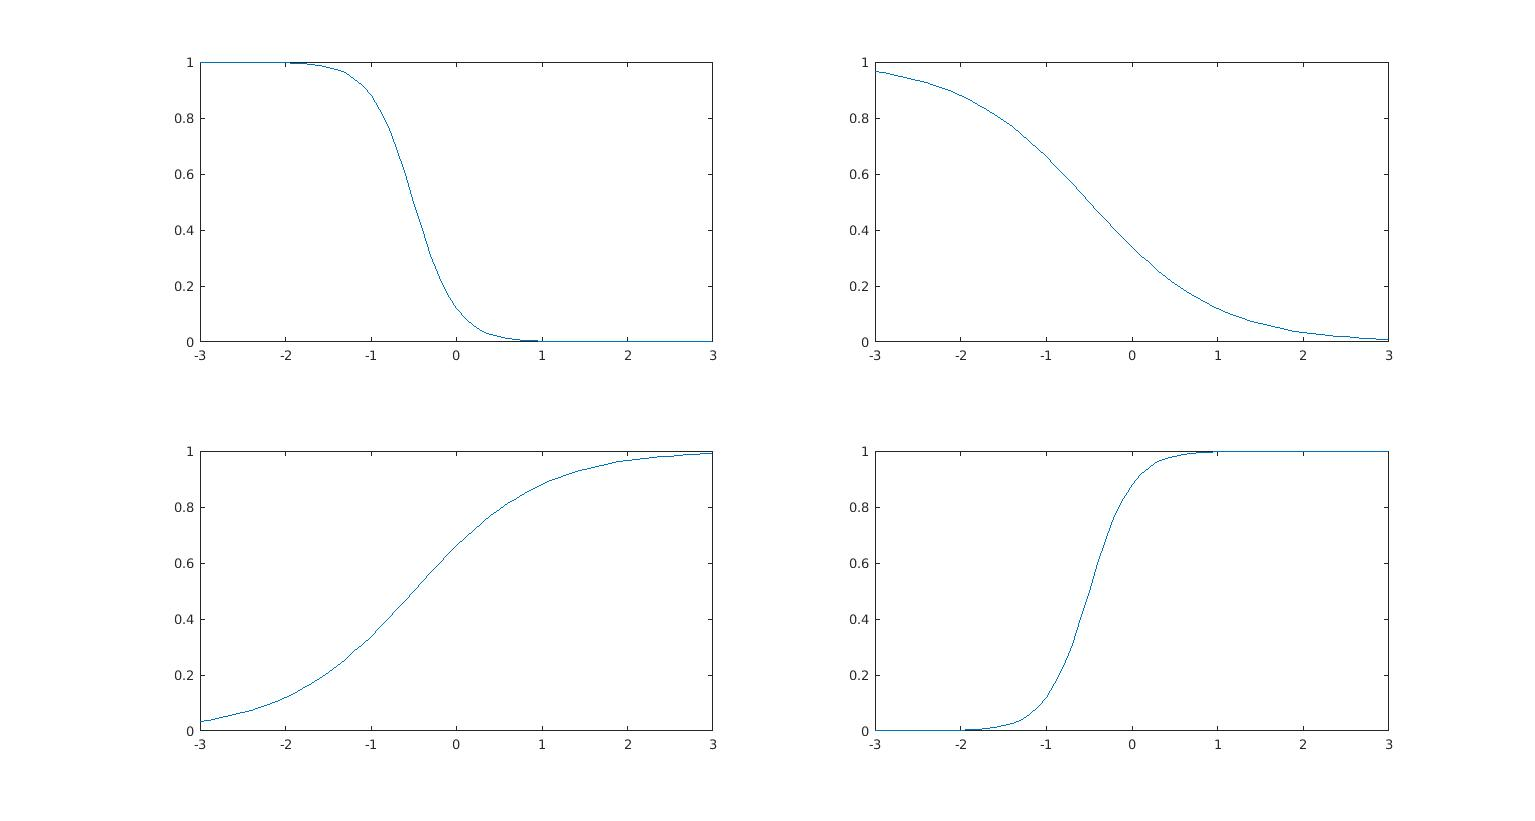
\includegraphics[width=0.75\textwidth]{./logits.jpg}\\
\vspace{-5mm}
Algunos ejemplos de funciones logit.
\end{center}
Se puede demostrar que el recorrido de cualquier funci\'on logit es siempre $]0,1[$. Esto permite utilizarla como funci\'on modelo de una probabilidad de un evento. Por ejemplo, considere que los datos
\begin{center}\small
\begin{tabular}{|l|c|c|c|c|c|c|c|c|c|c|c|c|}\hline
Edad &22   &23  &21  &28  &29 &18 &33 &34 &29 &20 &21& 23 \\\hline
Hijos &0 &1 &1 &2 &2 &0 &1 &1 &1 &2 &0 &0 \\\hline
\end{tabular}
\end{center}
representan la edad de 12 personas entre 20 y 35 a\~{n}os y la cantidad de hijos que cada uno tiene. Se puede pensar que la probabilidad de tener hijos es funci\'on de la edad, digamos $\pi(x)$. Para las personas de los datos enteriores, tendr\'iamos que
\begin{center}
$
\pi(22)=0, \quad 
\pi(23)=1, \quad 
\pi(21)=1, \quad 
\pi(28)=1, \quad 
\pi(29)=1, \quad 
\pi(18)=0, 
$\\
$
\pi(33)=1, \quad 
\pi(34)=1, \quad
\pi(29)=1, \quad 
\pi(20)=1, \quad 
\pi(21)=0, \quad 
\pi(23)=0, \quad 
$
\end{center}
As\'i, si proponemos que esta funci\'on de probabilidad sea una funci\'on logit, tendr\'iamos que para cada uno de estos datos
$$
\begin{array}{c|}
\displaystyle
\beta_0+\beta_1 22 = ln\left(\frac{\pi(22)}{1+\pi(22)}\right)
\displaystyle\\
\beta_0+\beta_1 23 = ln\left(\frac{\pi(23)}{1+\pi(23)}\right) \\
\vdots\\
\displaystyle
\beta_0+\beta_1 23 = ln\left(\frac{\pi(23)}{1+\pi(23)}\right)\\
\hline
\end{array}
$$
Debido al recorrido de la funci\'on logit y para que este sistema est\'e bien planteado, a los \'exitos y fracasos en las probabilidades anteriores, debemos reasignarles valores dentro del intervalo $]0,1[$, propongamos que $0.01$ y $0.09$ sean estas asignaciones respectivamente. Con esta modificaci\'on el problema anterior nos lleva al sistema
$$
\begin{array}{c|}
\displaystyle
\beta_0+22\beta_1  = ln\left(\frac{0.01}{1+0.01}\right)
\displaystyle\\
\beta_0+ 23\beta_1 = ln\left(\frac{0.99}{1+0.99}\right) \\
\vdots\\
\displaystyle
\beta_0+23\beta_1  = ln\left(\frac{0.01}{1+0.01}\right)\\
\hline
\end{array}
\rightarrow
\begin{bmatrix}
1 & 22\\
1 & 23 \\
\vdots & \vdots\\
1 & 23
\end{bmatrix}
\begin{bmatrix}
\beta_0\\\beta_1
\end{bmatrix}
=
\begin{bmatrix}
-4.5951\\
+4.5951\\
\vdots
-4.5951\\
\end{bmatrix}
$$
el cual tiene por soluci\'on en el sentido de m\'inimos cuadrados
$
\beta_0=-10.6567, \quad \beta_1=0.4859.
$
As\'i, con estos par\'ametros se determina la funci\'on de regresi\'on logit
\begin{center}
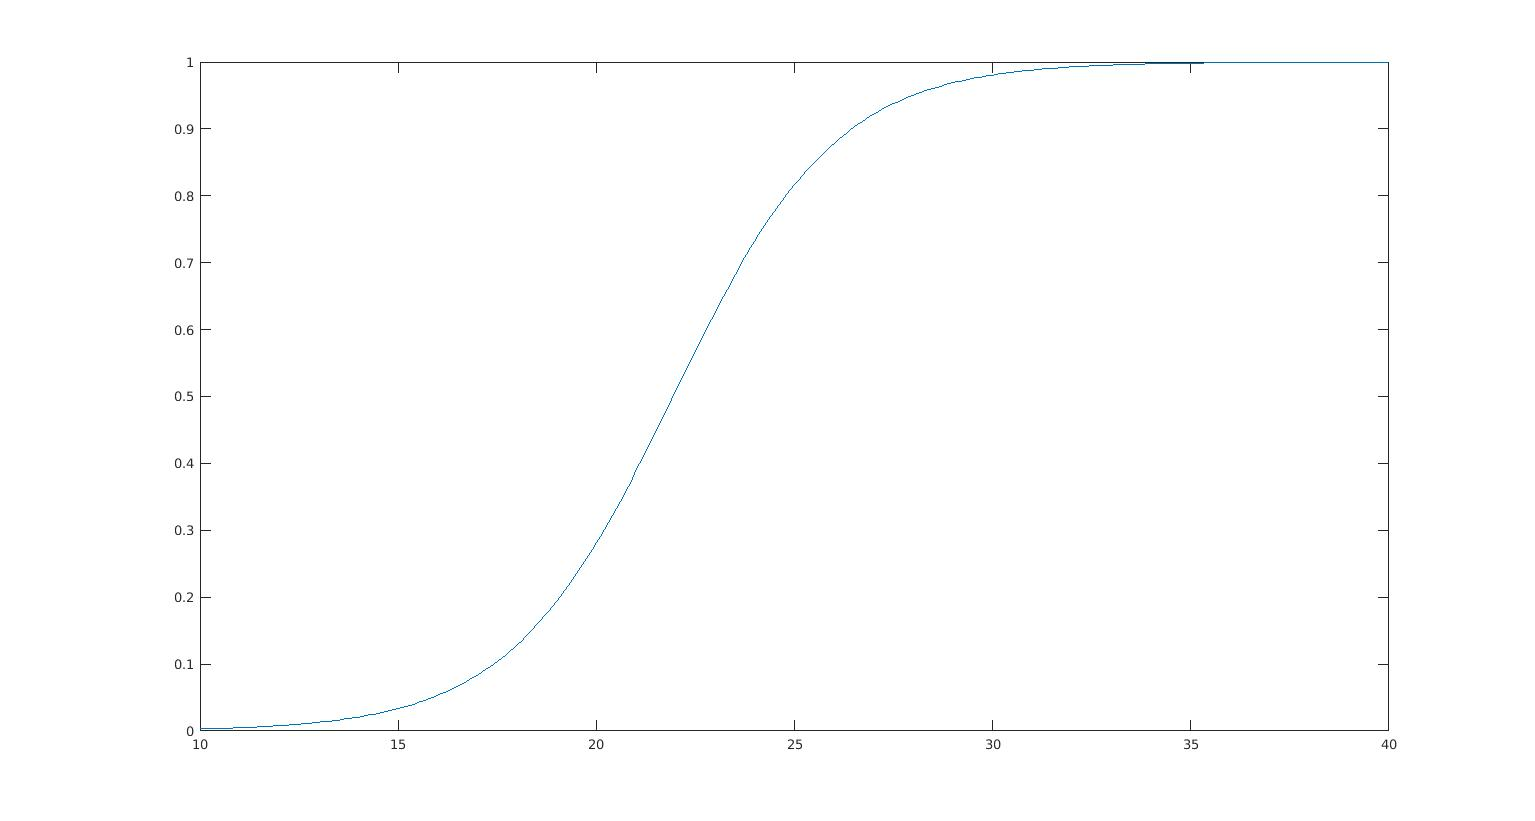
\includegraphics[width=0.75\textwidth]{./logitejemplo.jpg}\\
\end{center}
la cual nos permite concluir que a los 22 a\~{n}os, considerando este grupo de personas, existe una probabilidad 
$$
\pi(22)=\frac{e^{-10.6567_0+0.4859 \cdot 22}}{1-e^{-10.6567+0.4859 \cdot 22}}=0.5084 
$$
de tener hijos.

\subsection{Funciones peri\'odicas}
Algunas veces los datos pueden tener un comportamiento peri\'odico en el tiempo. En estos casos resulta emp\'iricamente mas adecuado utilizar como modelo de ajuste funciones que sean peri\'odicas.

Supongamos que $\{(x_i,y_i)\}_{i=0}^n$ son los puntos a los que queremos ajustarle una funci\'on del tipo
$$
f(x)=a_0+a_1cos(x)+a_2sen(x),
$$
en este caso, y similarmente a todos los ejemplos anteriores, una vez mas se llega a un sistema de ecuaciones
$$
\begin{array}{c|}
f(x_0) = y_0\\
f(x_1) = y_1\\
\vdots
f(x_n) = y_n\\
\hline
\end{array}
\rightarrow
\begin{bmatrix}
1 & cos(x_0) & sen(x_0)\\
1 & cos(x_1) & sen(x_1)\\
\vdots & \vdots & \vdots\\
1 & cos(x_n) & sen(x_n)\\
\end{bmatrix}
\begin{bmatrix}
a_0\\ a_1\\\ a_2
\end{bmatrix}
=
\begin{bmatrix}
y_0\\y_1\\\vdots \\y_n
\end{bmatrix}
$$
el cual, en general, podemos resolver mediante m\'inimos cuadrados. Creando as\'i una forma particular de funci\'on $f$ peri\'odica que mas se aproxima a todos los puntos.

Por ejemplo, considere los datos disponibles en 
\href{ftp://ftp.ing-mat.udec.cl/pub/ing-mat/asignaturas/521230/ejercicios/2018-1/puntos.mat}{puntos.mat}
este contiene dos variables \texttt{x} e \texttt{y} que representan el muestreo de una funci\'on peri\'odica como la del ejemplo. En un rutero de \matlab ensamble las matrices del sistema de ecuaciones descrito anteriormente para estos puntos y resu\'elvalo. Luego, cuando tenga esta soluci\'on interprete el vector obtenido. Con esto usted podr\'a graficar 
\begin{center}
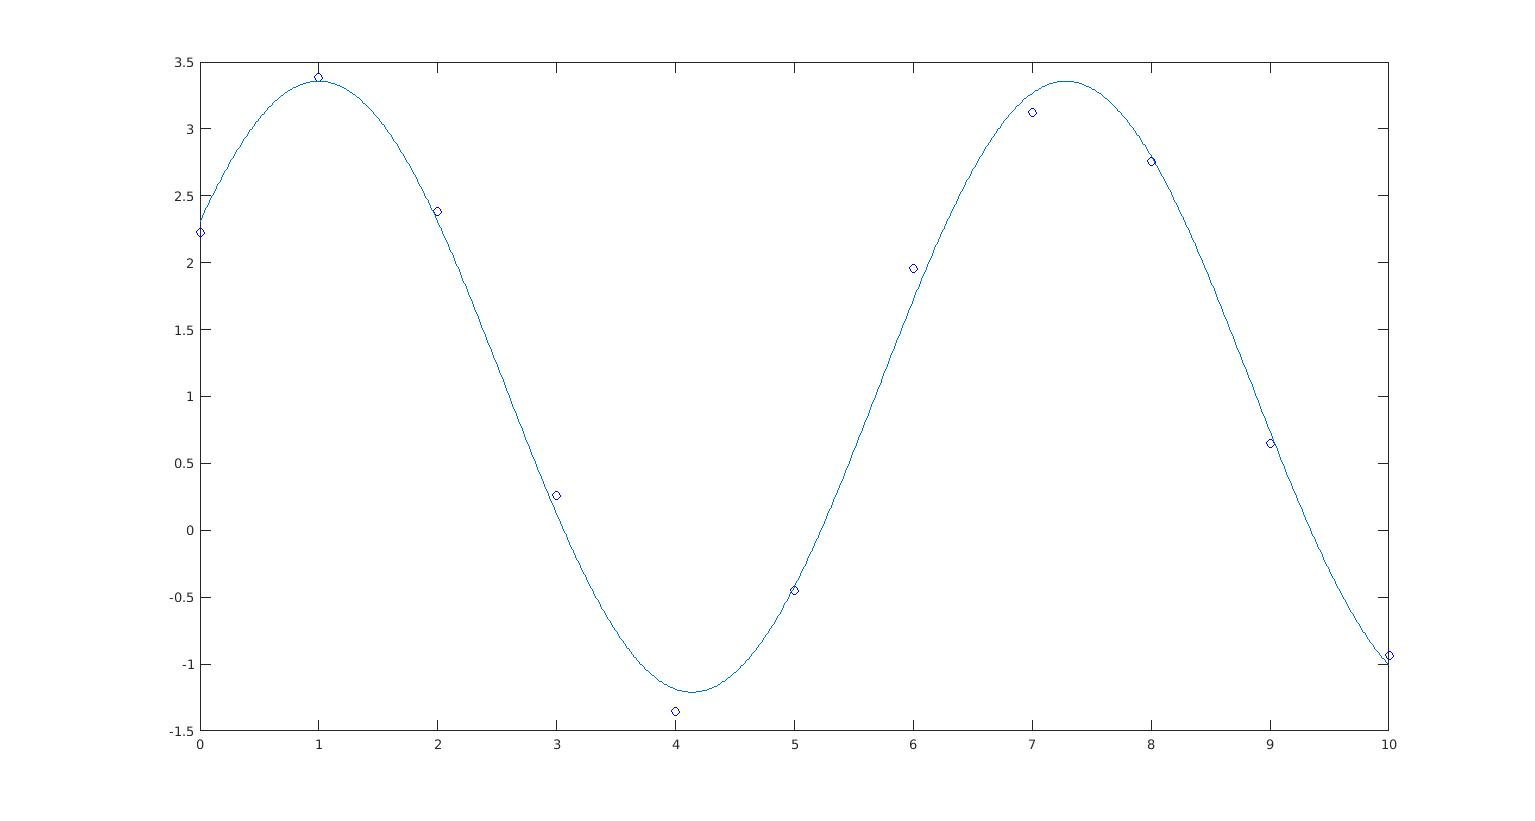
\includegraphics[width=0.75\textwidth]{./periodica.jpg}\\
\vspace{-5mm}
\end{center}
donde se observa que la funci\'on calculada se ajusta a los puntos.

\section{Ejercicios}
\begin{enumerate}
\item 
En un rutero llamado \texttt{interpolacion.m} cargue el archivo de \matlab
\href{ftp://ftp.ing-mat.udec.cl/pub/ing-mat/asignaturas/521230/ejercicios/2018-1/data.mat}{data.mat}
usando la funci\'on \texttt{load}. Este archivo contiene tiempo y longitud de las mediciones del movimiento de un resorte en cierto experimento.

En el rutero \texttt{interpolacion.m}
\begin{enumerate}
\item grafique los datos cargados usando la funci\'on \texttt{plot} con asteriscos azules,
\item grafique el polinomio interpolante de los datos cargados.
\end{enumerate}

\item La siguiente tabla
\begin{center}
\begin{tabular}{c|ccccc}
$x$ & -2 & -1 &  0  & 1 &  2\\\hline
$f(x)$& -25 & -4 & -1 & 8 & 47
\end{tabular}
\end{center}
corresponde a los valores de una cierta funci\'on $f$ en los puntos $-2,-1,0,1,2$.
\begin{enumerate}
\item Calcule, con ayuda del comando \texttt{polyfit} los polinomios $p_1 \in \mathcal{P}_1(\mathbb{R})$,
$p_2 \in {\mathcal P}_2(\mathbb{R})$, $p_3 \in {\mathcal P}_3(\mathbb{R})$, $p_4 \in {\mathcal P}_4(\mathbb{R})$, $p_5 \in {\mathcal P}_5(\mathbb{R})$
que mejor ajustan por m\'{\i}nimos 	cuadrados los datos en la tabla y complete

\begin{center}
\begin{tabular}{|c|}\hline
$p_1(x)=$ \hspace*{8cm}\\\hline	
$p_2(x)=$ \hspace*{8cm}\\\hline
$p_3(x)=$ \hspace*{8cm}\\\hline
$p_4(x)=$ \hspace*{8cm}\\\hline
$p_5(x)=$ \hspace*{8cm}\\\hline
\end{tabular}
\end{center}

\item Por cada uno de los polinomios determinados antes, grafique, en una misma
figura, al polinomio, evaluado en 100 puntos entre -2 y 2 y los puntos en la tabla. Para ello, averig\"ue con el comando \verb"help" c\'omo usar el comando \verb"polyval".

\item Haga un nuevo gr\'afico con los puntos en la tabla y el polinomio
$q(x) = x^5 -x^3 +3x^2 + 6x -1$, evaluado en 100 puntos
entre -2 y 2.

\item?`Cu\'ales de los polinomios $p_1, p_2, p_3, p_4, p_5, q$ interpolan los pares en la tabla?

\item Observe que $p_3$ y $p_4$ coinciden. ?`Contradice esto el teorema visto en clases sobre
existencia y unicidad del polinomio de interpolaci\'on?

\item Observe que $p_5$ y $q$ no coinciden. ?`Contradice esto
el teorema visto en clases sobre existencia y unicidad del
polinomio de interpolaci\'on?
			
	\end{enumerate}
            
\item Cargue usando la funci\'on de \matlab \texttt{load} el archivo 
\href{ftp://ftp.ing-mat.udec.cl/pub/ing-mat/asignaturas/521230/ejercicios/2018-1/dolar.mat}{dolar.mat}.
Este archivo contiene los valores del d\'olar durante algunos d\'ias. 

\begin{enumerate}
\item Grafique usando c\'irculos azules el valor del d\'olar por d\'ia.
\item Calcule y grafique el polinomio interpolante de los datos.
\item Identifique el fen\'omeno de Runge en este gr\'afico.
\item Calcule y grafique el spline c\'ubico de los datos.
\item Calcule y grafique la recta que mejor se ajusta a los datos.
\item Cree un rutero que calcule la funci\'on de la forma 
$$
f(x)=ax^3+bx+c, \quad a,b,c\in\mathbb{R}
$$
que mejor se ajuste a los datos. Grafique \'esta junto con los datos.
\item Compare los cuatro modelos de ajustes anterior en un mismo gr\'afico.
\end{enumerate}

\item Considere $f(x) = \ln(x)$.
	\begin{enumerate}
		\item \label{interppol} Determine, mediante el comando \Verb+polyfit+ de \matlab\, un polinomio que interpole a $f$ en los puntos
			$1, 2, 3$. Escoja el grado de este polinomio de forma que su existencia y unicidad est\'en aseguradas.
		\item Grafique, en un mismo gr\'afico, a la funci\'on $f$ y al polinomio calculado, evaluados en 200
			puntos entre 1 y 3. Recuerde que puede utilizar
			el comando \Verb+polyval+ para evaluar al polinomio. ?`C\'omo se reconoce en el gr\'afico que $p$ interpola a $f$, as\'{\i}
			como los puntos de interpolaci\'on?
		\item Grafique, en un mismo gr\'afico, los valores $|f(x_i) - p(x_i)|$ y
			\[
				\frac{1}{3!}\max_{x \in [1,\,3]} \left|f^{\prime\prime\prime}(x)\right|\left|(x_i-1)(x_i-2)(x_i-3)\right|
			\]
			con $x_i = 1 + ih,\;i=0,1,2,\ldots,100, \; h = \dfrac{1}{50}$.
			?`Se cumple
			\[
				\left|f(x_i)-p(x_i)\right| \le
					\frac{1}{3!}\max_{x \in [1,\,3]} \left|f^{\prime\prime\prime}(x)\right|\left|(x_i-1)(x_i-2)(x_i-3)\right|,\; i=0,1,2,\ldots,100\,\mbox{?}
			\]
	\end{enumerate}

\item Construya un rutero que dibuje un polinomio interpolante de un conjunto de datos y sus primeras dos derivadas en distintos gr\'aficos de una misma figura. Para esto ocupe la funci\'on \texttt{vander} y calcule expl\'icitamente los coeficientes del polinomio, luego derive estos polinomios. Finalmente, para anexar varios gr\'aficos dentro de una figura use la funci\'on \texttt{subplot}.

\item En el archivo 
\href{ftp://ftp.ing-mat.udec.cl/pub/ing-mat/asignaturas/521230/ejercicios/2018-1/pesoestatura.mat}{pesoestatura.mat} 
se encuentran los datos hist\'oricos de peso y estatura de dos hermanos gemelos nacidos el 24 de abril de 1987. Use la funci\'on \texttt{load} para leer el archivo, luego utilize la funci\'on \texttt{datenum}, para convertir las fechas de las primeras tres columnas en un n\'umero que representa el tiempo en d\'ias.

Luego haga dos gr\'aficos de sus pesos y estaturas versus el tiempo, dibuje en c\'irculos rojos los datos descargados Adem\'as incluya a estos datos sus ajustes lineales, polinomio de interpolaci\'on y spline c\'ubica. Incluya t\'itulo y leyenda de cada una de las funciones dibujadas.

\item En una hoja de papel delgada sobrepone una de tus manos, con un l\'apiz marca una cantidad de puntos finita, que te parezca adecuada, para representar el contorno de tu mano. En la ventana de comandos escribe las siguientes instrucciones
\begin{lstlisting}
figure('position',get(0,'screensize'))
axes('position',[0 0 1 1])
[x,y] = ginput;
\end{lstlisting}
Posiciona la hoja de papel con los puntos sobre la pantalla de tu computador y usa el mouse para seleccionar alguno de estos puntos (deberías poder ver a trav\'es de la hoja de papel la posici\'on del mouse), finalmente apreta la tecla enter. Luego graba estos datos usando el comando 
\begin{lstlisting}
save x,y;
\end{lstlisting}
Ahora imagina que estos vectores \texttt{x,y} son muestras de dos funciones $x,y:\mathbb{R}\rightarrow \mathbb{R}$, ejecuta una interpolaci\'on polinomial y splines c\'ubicos de estas funciones. Finalmente grafica en el plano la funci\'on que obtienes al interpolar la funci\'on $(x(t),y(t))$ y los puntos de los vectores \texttt{x,y}.

\item La funci\'on Gamma est\'a definida por
$$
\Gamma(x)=\int_0^\infty t^{x-1}e^{-t}dt, \quad x>0/
$$
Se sabe que cuando se eval\'ua en un natural $n \geq 1$, se tiene que 
$$
\Gamma(n)=(n-1)!
$$
en consecuencia, un conjunto de puntos de esta funci\'on son 
\begin{center}
\begin{tabular}{c|ccccc}
$x$ 	& 1 & 2	& 3 & 4 & 5 \\
\hline
$y$	& 1	& 1 & 2 & 6 & 24
\end{tabular}
\end{center}
\begin{enumerate}
\item Calcule el polinomio de grado cuatro que interpola estos puntos. Dibuje este polinomio y tambi\' en la funci\'on usando la funci\'on de \matlab \texttt{gamma}
\item Realize una interpolaci\'on por splines c\'ubicos de estos puntos, nuevamente dib\'ujenla junto con la funci\'on \texttt{gamma}.
\item \textquestiondown Cual de los dos interpolantes es mejor?,
\item \textquestiondown Cual de los dos interpolantes es mejor en el intervalo [1,2]?,
\end{enumerate}

\item La siguiente tabla relaciona el ordinal de un d\'ia del a\~no 2014 (d\'ia 1 = 1 de enero, d\'ia 30 = 30 de enero, d\'ia 57 = 26 de febrero, etc.) con la hora (UTC-3, expresada en minutos; esto es, 398 = 6:38, 427 = 7:07, 456 = 7:36, etc.) en la que amaneci\'o ese d\'ia en Concepci\'on:
\smallskip
\begin{center}\small
\begin{tabular}{|l|c|c|c|c|c|c|c|c|c|c|c|c|}\hline
D\'ia (ordinal)  &1   &30  &57  &88  &117 &135 &169 &197 &227 &255 &286 &311 \\\hline
Hora (minutos) &398 &427 &456 &484 &509 &525 &545 &543 &517 &478 &432 &402 \\\hline
\end{tabular}
\end{center}
\smallskip
%
Sobre estos datos se desea ajustar por cuadrados m\'inimos una funci\'on $m\colon\mathbb{R} \to \mathbb{R}$ de la forma
%
\begin{equation*}
m(d) = c_0 + \sum_{k=1}^3 c_k \cos\!\left(k \, d \, \frac{2\pi}{365}\right) + \sum_{k=1}^3 s_k \sen\!\left( k\, d \, \frac{2\pi}{365} \right),
\end{equation*}
%
\begin{enumerate}
\item %\label{it:func_trig_cols}
Escriba una funci\'on Matlab que reciba como entrada un vector columna $d$, una frecuencia angular
%\footnote{La frecuencia angular de un fen\'omeno se define como $2\pi$ veces su frecuencia.} 
$f \in \mathbb{R}$ y un n\'umero de onda m\'aximo $K \in \mathbb{N}$ y  devuelva la matriz de orden $n \times (2K+1)$
%
\begin{equation*}
\begin{pmatrix}
1 & \cos\!\left(d_1 f \right) & \cos\!\left(2 d_1 f \right) & \cdots & \cos\!\left(K d_1 f \right) & \sen\!\left(d_1 f \right) & \sen\!\left(2 d_1 f \right) & \cdots & \sen\!\left(K d_1 f \right)\vspace{1ex}\\
1 & \cos\!\left(d_2 f \right) & \cos\!\left(2 d_2 f \right) & \cdots & \cos\!\left(K d_2 f \right) & \sen\!\left(d_2 f \right) & \sen\!\left(2 d_2 f \right) & \cdots & \sen\!\left(K d_2 f \right)\\
\vdots & \vdots & \vdots && \vdots & \vdots & \vdots & & \vdots\\
1 & \cos\!\left(d_n f \right) & \cos\!\left(2 d_n f \right) & \cdots & \cos\!\left(K d_n f \right) & \sen\!\left(d_n f \right) & \sen\!\left(2 d_n f \right) & \cdots & \sen\!\left(K d_n f \right)
\end{pmatrix},
\end{equation*}
%
donde $n$ es la longitud de $d$.
Recuerde que en \matlab la funci\'on seno se llama \texttt{sin}.
\bigskip
\item Escriba un rutero Matlab que:
\begin{itemize}
\item Use la funci\'on construida en la parte anterior para ajustar los coeficientes $c_i$ y $s_i$, $i \in \{1, 2, r\}$, a los datos de la tabla mediante cuadrados m\'inimos.

\textbf{Indicaci\'on}: naturalmente $K = 3$ y $f = \frac{2\pi}{365}$

\item Calcule a qu\'e hora amaneci\'o el 25 de diciembre de 2014 (d\'ia 359 del a\~no) seg\'un la funci\'on $m$ ajustada 

\textbf{Indicaci\'on}:  una llamada a la funci\'on que usted escribi\'o anteriormente con $d$ igual a $\texttt{[359]}$ le puede ser \'util.
\end{itemize}
\end{enumerate}


\end{enumerate}

\vfill
\hfill Revisado a Semestre 2018--1
\end{document}
